\documentclass{beamer}
\usepackage{amsfonts,amsmath,oldgerm}
\usepackage{ragged2e}

\usetheme{sintef}

\newcommand{\testcolor}[1]{\colorbox{#1}{\textcolor{#1}{test}}~\texttt{#1}}

\usefonttheme[onlymath]{serif}

\titlebackground*{assets/background}

\newcommand{\hrefcol}[2]{\textcolor{cyan}{\href{#1}{#2}}}

\title{Aula Zero - Programa da Disciplina}
\subtitle{2023.1 - SPOPFDS - Prát. e Ferr. de Desenvolvimento de Software}
\course{Tecnologia em Análise e Desenvolvimento de Sistemas}
\author{\href{mailto:luiz.quirino@ifsp.edu.br}{Luiz \textbf{Quirino}}}
\IDnumber{luiz.quirino@ifsp.edu.br}



\begin{document}
\maketitle

%\begin{frame}
%
%      Este material é produzido utilizando \LaTeX\, baseado na SINTEF Presentation, disponibilizado sob licenciamento \hrefcol{https://creativecommons.org/licenses/by-nc/4.0/legalcode}{Creative Commons CC BY 4.0}
%
%\vspace{\baselineskip}

%In the following you find a brief introduction on how to use \LaTeX\ and the beamer package to prepare slides, based on the one written by \hrefcol{mailto:federico.zenith@sintef.no}{Federico Zenith} for \hrefcol{https://www.overleaf.com/latex/templates/sintef-presentation/jhbhdffczpnx}{SINTEF Presentation}

% This template is released under \hrefcol{https://creativecommons.org/licenses/by-nc/4.0/legalcode}{Creative Commons CC BY 4.0} license
%\end{frame}
\footlinecolor{sintefdarkgreen}

\section{Introdução}
\begin{frame}{Conceito de Terminal}\justifying
      O terminal, também conhecido como linha de comando, é uma interface de texto em um sistema operacional que permite que os usuários interajam com o computador por meio de comandos de texto.
  
      \vspace{0.5cm}
  
      Diferencia-se das interfaces gráficas por ser baseado em texto, sendo uma forma poderosa e flexível de comunicar-se com o sistema.
  \end{frame}
  \begin{frame}{História do Terminal}\justifying
      \begin{itemize}
          \item No início dos computadores: controle através de cartões perfurados.
          \item Surgimento de terminais de tubo de raios catódicos (CRT) e terminais impressores.
          \item Amplamente utilizados até a chegada das interfaces gráficas nos anos 70 e 80.
          \item Popularização dos computadores pessoais.
          \item Sistemas operacionais baseados em Unix destacaram os terminais de texto.
          \item Emuladores de terminais em computadores pessoais se tornaram predominantes.
      \end{itemize}
  \end{frame}
\section*{O que é um terminal}  
\begin{frame}\justifying
      \frametitle{Definição de Terminal}
      
      Um \textit{terminal} é uma interface de texto em um sistema operacional que permite aos usuários interagir com o computador usando comandos de texto. É uma forma poderosa de comunicação com o sistema, onde os comandos são digitados em uma linha de comando e o sistema responde com mensagens e resultados em texto.
\end{frame}
      

      \begin{frame}\justifying
            \frametitle{Definição de Terminal}
      Essa forma de interação com o computador é comum em sistemas operacionais baseados em texto, como Unix e Linux, onde os usuários podem executar comandos para realizar tarefas, gerenciar arquivos, executar programas e muito mais, tudo através de comandos de texto digitados em um terminal.
      
      \end{frame}

      \begin{frame}\justifying
            \frametitle{Definição de Terminal}
      Os terminais podem ser emulados em computadores pessoais, permitindo que eles se comportem como terminais clássicos, mesmo em sistemas operacionais com interfaces gráficas. Essa interface de linha de comando continua sendo uma ferramenta poderosa e amplamente utilizada em ambientes de desenvolvimento, administração de sistemas e computação em geral.
      
      \end{frame}
      
      \begin{frame}\justifying
            \frametitle{Diferenças entre Terminal e Interface Gráfica}
            
            \textbf{Interface Gráfica}
            \begin{itemize}
                \item Interativa e visual.
                \item Usa elementos gráficos como ícones, janelas e botões.
                \item Requer o uso de mouse e/ou teclado.
                \item Facilita a interação com o sistema por meio de cliques e gestos.
                \item Ações são executadas visualmente.
            \end{itemize}
      \end{frame}
            
      
            \begin{frame}\justifying
                  \frametitle{Diferenças entre Terminal e Interface Gráfica}
                           
            \textbf{Terminal}
            \begin{itemize}
                \item Interativa e baseada em texto.
                \item Usa comandos de texto para interagir com o sistema.
                \item Requer apenas o uso do teclado.
                \item Permite maior controle e flexibilidade sobre o sistema.
                \item Permite a execução de tarefas complexas com rapidez e eficiência.
            \end{itemize}
            
            A escolha entre usar uma Interface Gráfica ou um Terminal depende das necessidades e preferências do usuário. Ambos têm suas vantagens e são amplamente utilizados em diferentes cenários de computação.
            \end{frame}
\section{Evolução dos terminais}
\begin{frame}
      \frametitle{Terminais Físicos Antigos}
      
      No início da computação, os terminais eram dispositivos físicos separados do computador principal. Eles geralmente consistiam em monitores CRT (tubo de raios catódicos) conectados a sistemas centrais, como mainframes e minicomputadores.
      
      \begin{columns}
      \begin{column}{0.5\textwidth}
      \textbf{Características}
      \begin{itemize}
          \item Conectados ao computador central.
          \item Utilização de monitores CRT.
          \item Interação por meio de teclado.
          \item Respostas exibidas em texto na tela.
          \item Usados para acesso remoto ao computador central.
      \end{itemize}
      \end{column}
      
      \begin{column}{0.5\textwidth}
      \begin{figure}
          \centering
          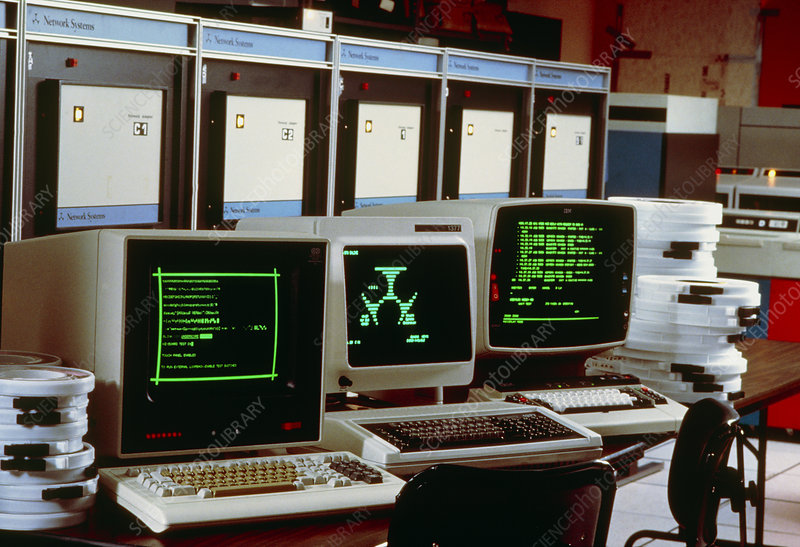
\includegraphics[width=0.6\textwidth]{assets/aula-tads-pfds/terminal_antigo.jpg}
          \caption{Exemplo de um terminal antigo com monitor CRT.}
      \end{figure}
      \end{column}
      \end{columns}
      
      \end{frame}
      \begin{frame}\justifying
            \frametitle{Terminais Físicos Antigos}
            Os terminais físicos permitiam que os usuários interagissem com o computador através de um teclado e recebessem as respostas em texto na tela.

      \end{frame}
     
      \begin{frame}
            \frametitle{Transição para Terminais Baseados em Software}
            
            \begin{columns}
            \begin{column}{0.6\textwidth}
            
            \begin{itemize}
                \item Facilidade de uso e acessibilidade.
                \item Conexão a sistemas remotos através de redes de computadores.
                \item Interação com sistemas remotos como se estivesse usando um terminal físico direto.
              
            \end{itemize}
            \end{column}
            
            \begin{column}{0.4\textwidth}
                \begin{itemize}
                    \item Maior flexibilidade e conveniência para os usuários.
                    \item Redução de custos, pois não requer hardware específico.
                \end{itemize}
            \end{column}
            \end{columns}
            \end{frame}

            \begin{frame}\justifying
                \frametitle{Benefícios dos Emuladores de Terminal}
                
                
                \begin{columns}\justifying
                \begin{column}{0.6\textwidth}
                    Com o avanço da tecnologia, os terminais físicos foram gradualmente substituídos por emuladores de terminais baseados em software. Os emuladores de terminal são programas que simulam as funções de um terminal físico, permitindo que um computador pessoal ou estação de trabalho se comporte como um terminal remoto.
                \end{column}
                
                \begin{column}{0.4\textwidth}
                \begin{figure}
                    \centering
                    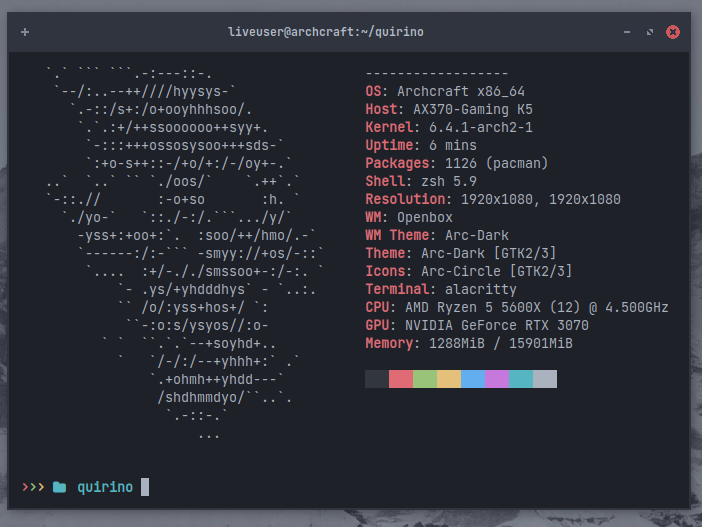
\includegraphics[width=0.8\textwidth]{assets/aula-tads-pfds/terminal_emulador.png}
                    \caption{Exemplo de um emulador de terminal baseado em software.}
                \end{figure}
                \end{column}
                \end{columns}
                \end{frame}

            \begin{frame}\justifying
                  \frametitle{Benefícios dos Emuladores de Terminal}
                  Essa transição possibilitou que os usuários se conectassem a sistemas remotos e interagissem com eles como se estivessem usando um terminal físico direto.
            \end{frame}
            
            
            

\begin{frame}[fragile]{Imagem do dia}

        \begin{figure}[H]
            \centerline{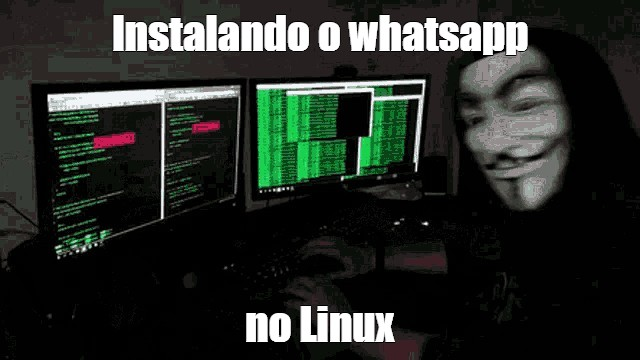
\includegraphics[width=0.5\textwidth]{assets/imagem-do-dia/terminal-hascker.jpg}}
            
        \end{figure}
\end{frame}


\footlinecolor{}

\backmatter
\end{document}
